% Figure S1 (V9): (a) trust chain of one data object; (b) event-identity slot transitions under Rule L, with the
% authorized reviewed-release transitions from LOST (dashed, marked R) as in Table S3.
% Drawn at final size: included at scale 1 in the supplement text width (17.4 cm); titles 9 pt, all other text 8 pt;
% notation as in the article (origin signature sigma_o, relay signature sigma_w; the checkpoint is a signed Merkle
% root). All line breaks are explicit, so no word is hyphenated inside a box. Dispositions are written in capitals,
% as in the article (Algorithm 1), at the full 8 pt size.
\documentclass[tikz,border=2pt]{standalone}
\usepackage[T1]{fontenc}
\usepackage{mathpazo}
\usepackage{amsmath}
\usetikzlibrary{positioning,arrows.meta,fit,backgrounds,calc}
\definecolor{acc}{HTML}{2F5D8A}\definecolor{ok}{HTML}{2E7D32}\definecolor{bad}{HTML}{B3261E}\definecolor{warn}{HTML}{8A5F00}
\tikzset{
 ev/.style={draw=black!70,rounded corners=2pt,fill=acc!7,align=center,font=\footnotesize,inner sep=2.5pt,
            minimum width=25.5mm,minimum height=21mm},
 flow/.style={-{Latex[length=2mm]},thick,black!70},
 st/.style={draw=black!75,thick,rounded corners=7pt,fill=white,font=\small\bfseries,minimum width=26mm,
            minimum height=8.5mm,align=center},
 tr/.style={-{Latex[length=2mm]},thick},
 rr/.style={-{Latex[length=2mm]},thick,dashed,acc},
 lab/.style={font=\footnotesize,align=center,inner sep=1.5pt},
 ptitle/.style={font=\small\bfseries,anchor=west,inner sep=0pt}
}
\begin{document}
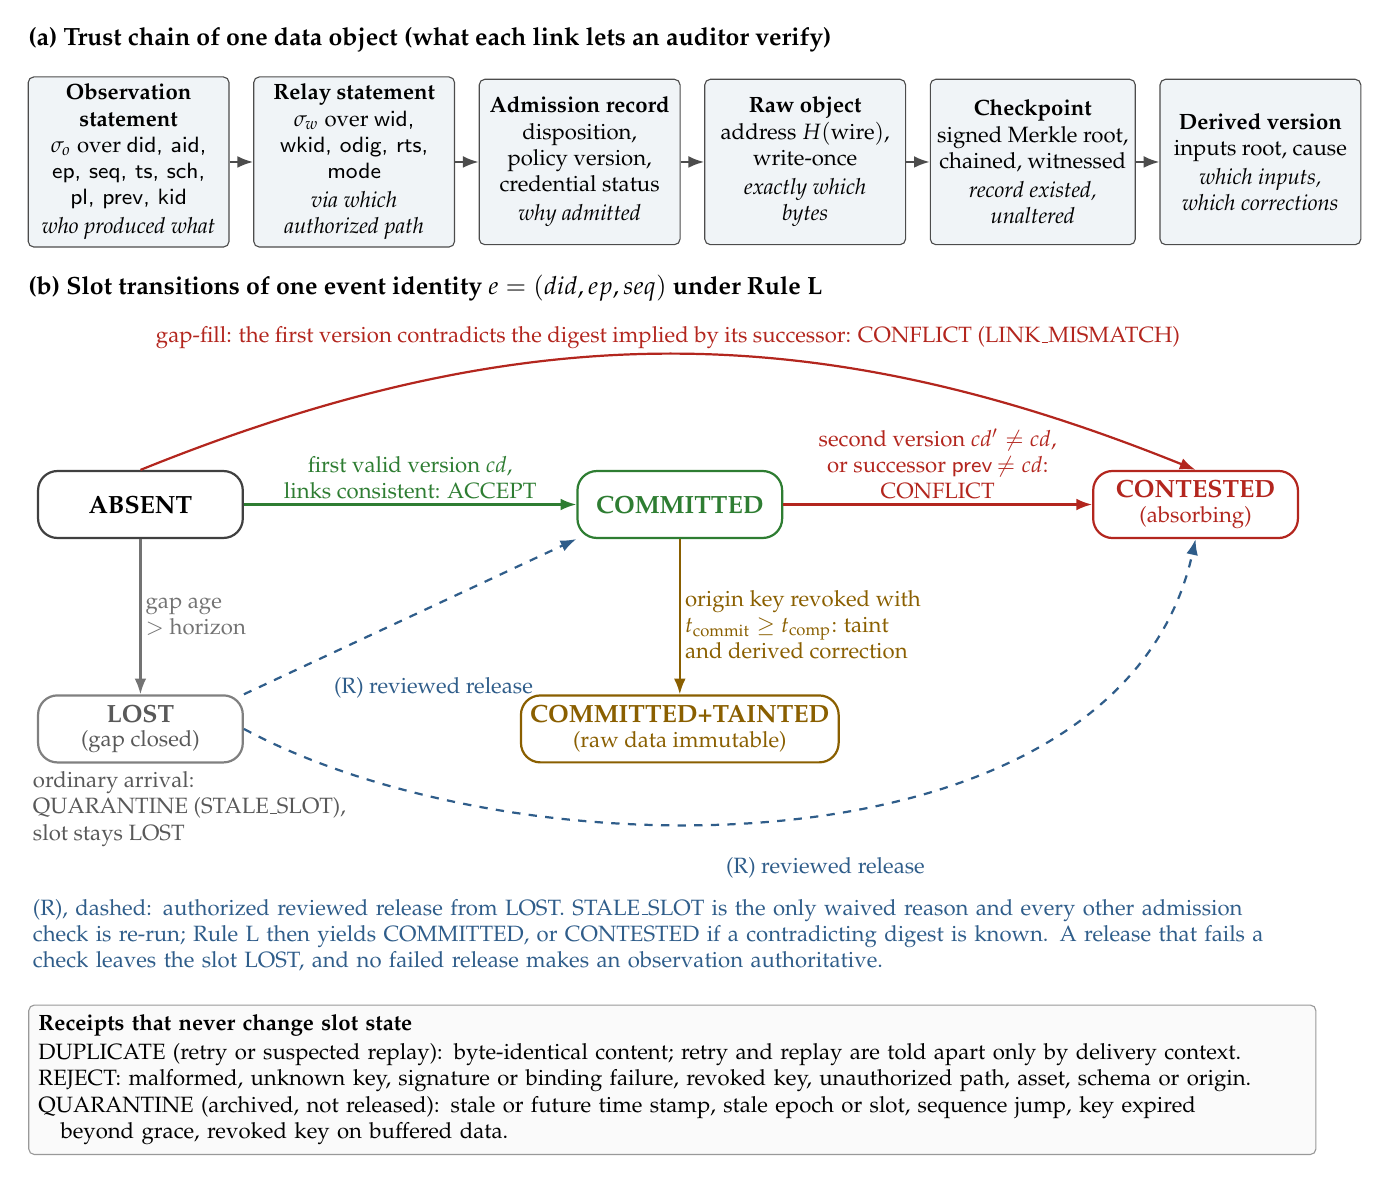
\begin{tikzpicture}
% ===================== (a) trust chain
\node[ptitle] at (-1.28,1.55) {(a) Trust chain of one data object (what each link lets an auditor verify)};
\node[ev] (o) at (0,0) {\textbf{Observation}\\\textbf{statement}\\$\sigma_o$ over \textsf{did, aid,}\\\textsf{ep, seq, ts, sch,}\\\textsf{pl, prev, kid}\\[1pt]\emph{who produced what}};
\node[ev,right=3mm of o] (r) {\textbf{Relay statement}\\$\sigma_w$ over \textsf{wid,}\\\textsf{wkid, odig, rts,}\\\textsf{mode}\\[1pt]\emph{via which}\\\emph{authorized path}};
\node[ev,right=3mm of r] (a) {\textbf{Admission record}\\disposition,\\policy version,\\credential status\\[1pt]\emph{why admitted}};
\node[ev,right=3mm of a] (w) {\textbf{Raw object}\\address $H(\mathrm{wire})$,\\write-once\\[1pt]\emph{exactly which}\\\emph{bytes}};
\node[ev,right=3mm of w] (c) {\textbf{Checkpoint}\\signed Merkle root,\\chained, witnessed\\[1pt]\emph{record existed,}\\\emph{unaltered}};
\node[ev,right=3mm of c] (d) {\textbf{Derived version}\\inputs root, cause\\[1pt]\emph{which inputs,}\\\emph{which corrections}};
\draw[flow] (o) -- (r);
\draw[flow] (r) -- (a); \draw[flow] (a) -- (w); \draw[flow] (w) -- (c); \draw[flow] (c) -- (d);
% ===================== (b) slot state machine
\begin{scope}[yshift=-4.35cm]
\node[ptitle] at (-1.28,2.75) {(b) Slot transitions of one event identity $e=(did,ep,seq)$ under Rule L};
\node[st] (A) at (0.15,0) {ABSENT};
\node[st,draw=ok,text=ok] (C) at (7.0,0) {COMMITTED};
\node[st,draw=bad,text=bad] (X) at (13.55,0) {CONTESTED\\[-2pt]{\footnotesize\mdseries(absorbing)}};
\node[st,draw=warn,text=warn] (T) at (7.0,-2.85) {COMMITTED+TAINTED\\[-2pt]{\footnotesize\mdseries(raw data immutable)}};
\node[st,draw=black!50,text=black!65] (L) at (0.15,-2.85) {LOST\\[-2pt]{\footnotesize\mdseries(gap closed)}};
\node[lab,anchor=north west,align=left,text=black!65] at (-1.275,-3.33) {ordinary arrival:\\QUARANTINE (STALE\_SLOT),\\slot stays LOST};
\draw[tr,ok] (A) -- node[lab,above,text=ok]{first valid version $cd$,\\links consistent: ACCEPT} (C);
\draw[tr,bad] (C) -- node[lab,above,text=bad]{second version $cd'\neq cd$,\\or successor \textsf{prev}$\,\neq cd$:\\CONFLICT} (X);
\draw[tr,bad] (A.north) to[out=22,in=158] node[lab,pos=0.5,above,text=bad]{gap-fill: the first version contradicts the digest implied by its successor: CONFLICT (LINK\_MISMATCH)} (X.north);
\draw[tr,warn] (C) -- node[lab,right,text=warn,align=left,pos=0.55]{origin key revoked with\\$t_\mathrm{commit}\ge t_\mathrm{comp}$: taint\\and derived correction} (T);
\draw[tr,black!55] (A) -- node[lab,right,align=left]{gap age\\$>$ horizon} (L);
\draw[rr] (L.north east) -- (C.south west);
\node[lab,text=acc,anchor=west] at (2.55,-2.33) {(R) reviewed release};
\draw[rr] (L.east) .. controls (5.0,-4.75) and (12.6,-4.75) .. (X.south);
\node[lab,text=acc,anchor=north] at (8.85,-4.42) {(R) reviewed release};
\node[lab,text=acc,align=left,anchor=north west,text width=161mm] at (-1.275,-4.95)
{(R), dashed: authorized reviewed release from LOST. STALE\_SLOT is the only waived reason and every other admission check is re-run; Rule L then yields COMMITTED, or CONTESTED if a contradicting digest is known. A release that fails a check leaves the slot LOST, and no failed release makes an observation authoritative.};
\node[draw=black!40,rounded corners=2pt,font=\footnotesize,align=left,anchor=north west,fill=black!2,inner sep=3.5pt,
      text width=161mm] at (-1.275,-6.35)
{\textbf{Receipts that never change slot state}\\[1pt]
DUPLICATE (retry or suspected replay): byte-identical content; retry and replay are told apart only by delivery context.\\
REJECT: malformed, unknown key, signature or binding failure, revoked key, unauthorized path, asset, schema or origin.\\
QUARANTINE (archived, not released): stale or future time stamp, stale epoch or slot, sequence jump, key expired\\
\quad beyond grace, revoked key on buffered data.};
\end{scope}
\end{tikzpicture}
\end{document}
